\documentclass[defaultpackages]{simplereport}
\usepackage{float}
\usepackage{listings}
\usepackage[]{enumitem}
\usepackage{bm}
\usepackage{tikz}
\usetikzlibrary{arrows,automata,positioning}
\title{Oblig 2}
\author{Åsmund Aqissiaq Arild Kløvstad}
\course[INF210]{Modelling of Computing}

\newcommand{\Z}{\mathbb{Z}}
\newcommand{\N}{\mathbb{N}}
\newcommand{\R}{\mathbb{R}}
\newcommand{\Q}{\mathbb{Q}}
\newcommand{\C}{\mathbb{C}}
\newcommand{\powerset}[1]{\mathcal{P}(#1)}

\lstset{
  basicstyle=\itshape,
  xleftmargin=3em,
  mathescape,
  literate={->}{$\rightarrow$}{2}
           {l}{$\lambda$}{1}
}

\begin{document}
\maketitle{}
\section*{main.pdf 5.7}
\paragraph{\textbf{4)}} This exercise is about the language of balanced
parentheses \[D = \{\mathbf{u} \in \Sigma^* \mid \text{all prefixes contain at
  least as many ['s as ]'s, and the total number of ['s equal the number of ]'s}\}\]
\begin{itemize}[label=]
  \item \textbf{a)} List all words in $D$ of length 6.\\ There are 5:
    $[ [ [ ] ] ], [ ] [ [ ] ], [ [ ] ] [ ], [ [ ] [ ] ] \text{ and } [ ] [ ] [
    ]$.
    
  \item \textbf{b)} Show that the language of all words of $D$ with length at
    most $n$ is regular for any fixed $n$.\\
    All finite languages are regular since they can be constructed by a finite
    number of concatenations and unions of singleton languages. This language is finite and therefore
    regular.
    
  \item \textbf{c)} Is the Dyck language of depth at most 3 regular? (Depth is
    the maximal number of nested parentheses)\\
    This restricted language is recognized by the following finite automaton:
  \begin{figure}[H]
     \centering
     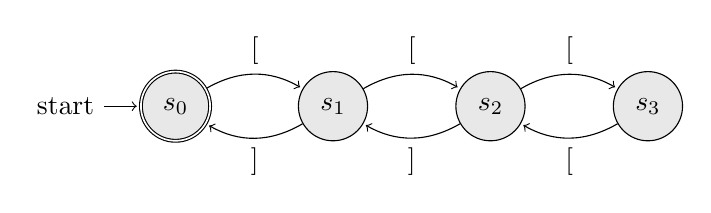
\begin{tikzpicture}[shorten >=1pt,node distance=2cm,on grid,auto]
       \tikzstyle{every state}=[fill={rgb:black, 1;white,10}]

       \node[state, initial, accepting] (s_0)                {$s_0$};
       \node[state]          (s_1) [right of=s_0] {$s_1$};
       \node[state]          (s_2) [right of=s_1] {$s_2$};
       \node[state]          (s_3) [right of=s_2] {$s_3$};

       \path[->]
       (s_0) edge [bend left] node {[} (s_1)
       (s_1) edge [bend left] node {[} (s_2)
             edge [bend left] node {]} (s_0)
       (s_2) edge [bend left] node {[} (s_3)
             edge [bend left] node {]} (s_1)
       (s_3) edge [bend left] node {[} (s_2);
     \end{tikzpicture}
  \end{figure}
  Since it is recognized by a finite automaton, it is regular.
  
\item \textbf{d)} Is the Dyck language of depth at most $n$ for any fixed $n$
  regular?\\
  We can construct a finite automaton like the one above for any fixed $n$ with
  $n+1$ states. By the same argument as before, this language is also regular.

\item \textbf{e)} Is the Dyck language regular?\\
  No. The language consisting of simply nested parentheses $\{[^n]^n \mid n \in \N\}$ is contained in
  the Dyck language. This is isomorphic to $\{a^nb^n \mid n \in \N\}$ which is
  known to be non-regular so the Dyck language is also non-regular.

\item \textbf{f)} An inductive definition of the Dyck language is given by:
  \[\lambda \in D'\]
  \[\mathbf{u}, \mathbf{v} \in D' \implies \mathbf{uv} \in D'\]
  \[\mathbf{w} \in D' \implies [\mathbf{w}] \in D'\]
  Show that these two definitions are equal.\\\\

  We will show the equality in two steps. First $D' \subseteq D$ by induction on
  the length of words $k$. As a base step for $k=0$, $\lambda \in D$ and also in
  $D'$ by definition. We form the induction hypothesis $\lvert \mathbf{w} \rvert
  \leq k,  \mathbf{w} \in D' \implies \mathbf{w} \in D$. Now we assume it holds for $k-1$ and
  show it also holds for $k$.\\
  Consider $\mathbf{w} \in D'$ of length $k$. Since it is in $D'$, either
  $\mathbf{w} = [\mathbf{w'}]$ or $\mathbf{w} = \mathbf{uv}$ for some
  $\mathbf{u,v, w'} \in D'$. In the first case $\lvert \mathbf{w'} \rvert \leq
  k$, so $\mathbf{w'}$ is in $D$ by the induction hypothesis and so $\mathbf{w}$
  is as well. In the second case $\lvert \mathbf{u} \rvert, \lvert \mathbf{v}
  \rvert < k$ (since we have used the rule to construct $\mathbf{w}$ from
  smaller parts) and hence in $D$ by the induction hypothesis. Since both are in
  $D$, they have an equal number of opening and closing parentheses, and so does
  $\mathbf{w}$ so it is in $D$.\\\\

  Secondly we show $D \subseteq D'$.
\end{itemize}

\section*{Textbook 3.3}
  Exercise 3) and 4) use the procedure described by the text book in section 3.3
  to mark pairs of states that cannot be collapsed, and then collapsing the
  remaining pairs.
\begin{itemize}[label=]
\item \textbf{3)} with one step labelled "a" from s4 to s2\\\\
  Step one marks $\{s_0, s_2\}, \{s_0, s_4\}, \{s_1, s_2\}, \{s_1, s_4\}, \{s_2,
  s_3\}, \{s_3, s_4\}$.\\
  Step two marks $\{s_0, s_1\}$ and $\{s_0, s_3\}$. The final two pairs are not
  marked in step three and we collapse $\{s_1, s_3\}$ and $\{s_2, s_4\}$
  resulting in the minimal automata in figure \ref{fig:3.3.3a}.
  \begin{figure}[H]
     \centering
     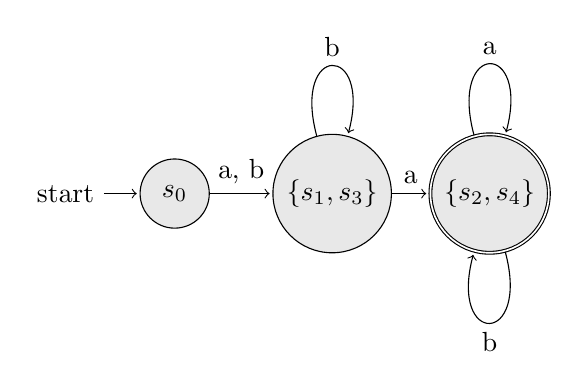
\begin{tikzpicture}[shorten >=1pt,node distance=2cm,on grid,auto]
       \tikzstyle{every state}=[fill={rgb:black, 1;white,10}]

       \node[state, initial] (s_0)                {$s_0$};
       \node[state]          (s_1) [right of=s_0] {$\{s_1, s_3\}$};
       \node[state,accepting](s_2) [right of=s_1] {$\{s_2, s_4\}$};

       \path[->]
       (s_0) edge [] node {a, b} (s_1)
       (s_1) edge [loop above] node {b} ()
             edge node {a} (s_2)
       (s_2) edge [loop above] node {a} ()
             edge [loop below] node {b} ();
     \end{tikzpicture}
     \caption{Minimal automata with ``a''-step from $s_4$ to $s_2$}
     \label{fig:3.3.3a}
  \end{figure}
\item \textbf{3)} as given\\\\
  Same as above, but this time step two also marks $\{s_2, s_4\}$ and only
  $\{s_1, s_3\}$ is collapsed resulting in figure \ref{fig:3.3.3b}
  \begin{figure}[H]
     \centering
     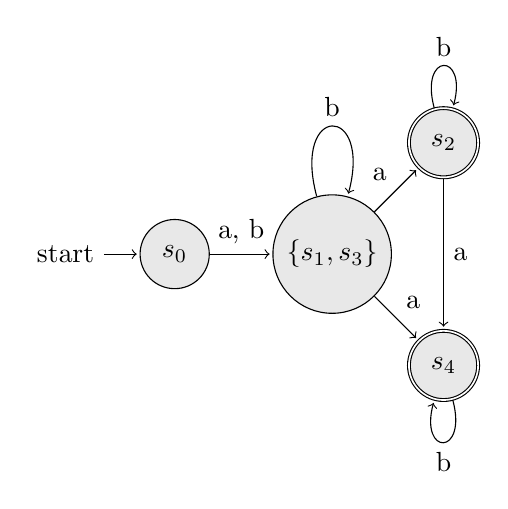
\begin{tikzpicture}[shorten >=1pt,node distance=2cm,on grid,auto]
       \tikzstyle{every state}=[fill={rgb:black, 1;white,10}]

       \node[state, initial] (s_0)                {$s_0$};
       \node[state]          (s_1) [right of=s_0] {$\{s_1, s_3\}$};
       \node[state,accepting](s_2) [above right of=s_1] {$s_2$};
       \node[state,accepting](s_3) [below right of=s_1] {$s_4$};

       \path[->]
       (s_0) edge [] node {a, b} (s_1)
       (s_1) edge [loop above] node {b} ()
             edge node {a} (s_2)
             edge node {a} (s_3)
       (s_2) edge [loop above] node {b} ()
             edge [] node {a} (s_3)
       (s_3) edge [loop below] node {b} ();
     \end{tikzpicture}
     \caption{Minimal automata as given}
     \label{fig:3.3.3b}
  \end{figure}
\item \textbf{4)}\\\\
  Step one marks $\{s_0, s_1\}, \{s_0, s_2\}, \{s_1, s_3\}, \{s_2, s_3\}$.\\
  Step two marks $\{s_1, s_3\}$ and $\{s_0, s_3\}$ is collapsed.
  \begin{figure}[H]
     \centering
     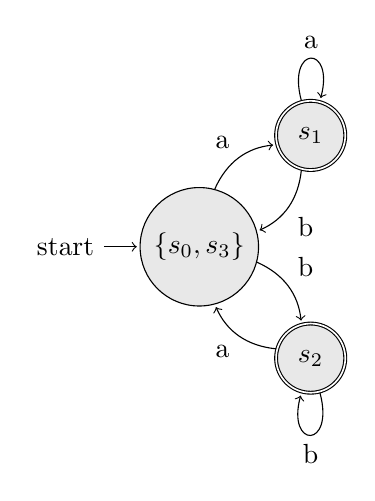
\begin{tikzpicture}[shorten >=1pt,node distance=2cm,on grid,auto]
       \tikzstyle{every state}=[fill={rgb:black, 1;white,10}]

       \node[state, initial] (s_0)                {$\{s_0, s_3\}$};
       \node[state,accepting](s_1) [above right of=s_0] {$s_1$};
       \node[state,accepting](s_2) [below right of=s_0] {$s_2$};

       \path[->]
       (s_0) edge [bend left] node {a} (s_1)
             edge [bend left] node {b} (s_2)
       (s_1) edge [loop above] node {a} ()
             edge [bend left] node {b} (s_0)
       (s_2) edge [loop below] node {b} ()
             edge [bend left] node {a} (s_0);
     \end{tikzpicture}
     \label{fig:3.3.4}
     \caption{Minimal automata 4)}
  \end{figure}
 \item \textbf{6)} Find minimal automaton for $a(b \mid c)^*bb^*$
  \begin{figure}[H]
     \centering
     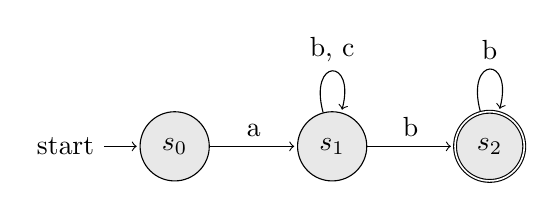
\begin{tikzpicture}[shorten >=1pt,node distance=2cm,on grid,auto]
       \tikzstyle{every state}=[fill={rgb:black, 1;white,10}]

       \node[state, initial] (s_0)                {$s_0$};
       \node[state](s_1) [right of=s_0] {$s_1$};
       \node[state,accepting](s_2) [right of=s_1] {$s_2$};

       \path[->]
       (s_0) edge [] node {a} (s_1)
       (s_1) edge [loop above] node {b, c} ()
             edge [] node {b} (s_2)
       (s_2) edge [loop above] node {b} ();
     \end{tikzpicture}
     \caption{Minimal automaton for $a(b \mid c)^*bb^*$}
  \end{figure}
\end{itemize}
\section*{Textbook 3.4}
\begin{itemize}[label=]
  \item \textbf{6)} Determine whether the language $\{\mathbf{ww} \mid
    \mathbf{w} \in \Sigma^*, \lvert \Sigma \rvert = 2\}$ is regular.\\
    \\
    Assume regular. Then by pumping lemma there exists an $n > 0$ such that for
    any word $\mathbf{xyz}$ in the language of length $n$ or greater,
    $\mathbf{x}\mathbf{y}^k\mathbf{z}$ is also in the language for all $k$.\\
    We consider $\mathbf{w} \in \Sigma^*$ such that $\lvert \mathbf{w} \rvert =
    n$ and say $\mathbf{w} = \mathbf{uv}$ with distinct $\mathbf{u}, \mathbf{v}$
    without loss of generality. Then $\mathbf{ww}$ is large enough for the pumping lemma and in the
    language by construction. Now let $\mathbf{ww} = \mathbf{xyz}$ in order to
    apply the pumping lemma. There are two ways this could split $\mathbf{ww}$: either $\mathbf{x} = \mathbf{w} =
    \mathbf{yz}$ or $\mathbf{y} = \mathbf{vu}$, splitting $\mathbf{w}$.\\
    In the first case $\mathbf{y}^k\mathbf{z} \neq \mathbf{w}$ for $k \neq 1$
    and the pumping lemma does not hold. (More precisely they are not
    \textit{necessarily} equal for an arbitrary $\mathbf{w}$).\\
    In the second case $\mathbf{x}\mathbf{y}^k\mathbf{z} =
    \mathbf{u}\mathbf{vu}^k\mathbf{v}$. For $k = 0$ we have $\mathbf{uv}$, which
    is certainly not in the language (assuming distinct $\mathbf{u},
    \mathbf{v}$) and so the pumping lemma does not hold.\\
    We conclude that the language is not regular.
  \item \textbf{7)} Determine whether the language $\{a^{2n} \mid n \geq 1\}$ is
    regular.\\\\
    We note that the language is described by the regular expression $(aa)^+$
    and conclude it is regular.
  \item \textbf{10)} Determine whether the language $\{\mathbf{ww}^R \mid
    \mathbf{w} \in \{a, b\}^*, \lvert \mathbf{w} \rvert \leq 3\}$ is
    regular.\\\\
    The language is finite, and therefore regular. It is described by the
    (exhaustive) regular expression ${aaaaaa} \mid {bbbbbb} \mid
    {abaaba} \mid {baaaab} \mid {aabbaa} \mid {aaaa}
    \mid {bbbb} \mid {abba} \mid {baab} \mid {aa} \mid {bb}$.
\end{itemize}
\section*{Textbook 3.5}
\begin{itemize}[label=]
  \item \textbf{1)} Prove there is an algorithm to decide if a regular language $L = \Sigma^*$\\\\
    We construct a 3-step algorithm based on the observation that $\Sigma^*
    \setminus \Sigma^* = \emptyset$
    \begin{enumerate}
    \item Construct a finite automaton $M_L$ accepting L
    \item Swap final and non-final states of $M_L$ to obtain an automaton for the complement of $L = \Sigma^* \setminus L$.
    \item For each final state in $M_{\Sigma^* \setminus L}$, check if reachable
      from initial state. If yes, then $L \neq \Sigma^*$. If no final states
      are reachable then $L = \Sigma^*$.
    \end{enumerate}
   This algorithm will terminate since $M_L$ is finite and hence $M_{\Sigma^*
     \setminus L}$ is finite. It produces the correct answer because $\Sigma^*
   \setminus L = \emptyset$ if and only if $L = \Sigma^*$
  \item \textbf{6)} Prove there is an algorithm for determining if there is a
    word in a regular language that begins with a given letter.\\\\
    Assume we have a finite automaton $M_L$ accepting $L$. Then for each state
    $q_i$ reachable from $q_0$ by the given letter and each final state $f_i$:
    if $f_i$ is reachable from $q_i$, return ``yes''. Then if we exhaust the
    search, return ``no''.\\
    This algorithm will terminate since $M_L$ is final. It gives the correct
    answer because any accepting path for a word starting with the given letter
    must start with that letter and end in a final state.
  \item \textbf{7)} Prove there is an algorithm to determine if a regular
    language contains a word of even length.\\\\
    We construct a 2-step algorithm based on the observation that any even
    number is a multiple of 2, and the assumption that we can find a path
    between two nodes in a graph. We also assume a finite automaton $M_L$
    accepting $L$:
    \begin{enumerate}
      \item construct a graph $G$ such that $V(G) = Q$ and $E(G) = \{(q_i, q_j)
        \mid \text{there is a path of length 2 from} q_i \text{to} q_j \text{in}
        M_L\}$
       \item for each final state $f_i$, look for a path from $q_0$ to $f_i$. If
         such a path exists return ``yes'', otherwise return ``no''. 
      \end{enumerate}
   This algorithm gives the right answer because if a path exists between $q_i$
   and $q_j$ in $G$, then it also exists in $M_L$ and a path of length $n$
   exists in $G$ if and only if a path of length $2n$ exists in $M_L$
\end{itemize}
\section*{Textbook 3.6}
\begin{itemize}[label=]
  \item \textbf{18)} Construct a pushdown automaton accepting $L =
    \{\textbf{w}c\textbf{w}^r \mid \textbf{w} \in \{a, b\}^*\}$.\\\\
    Use PDA model with empty stack-acceptance and stack alphabet $\{\alpha, \beta\}$.
    \begin{figure}[H]
     \centering
     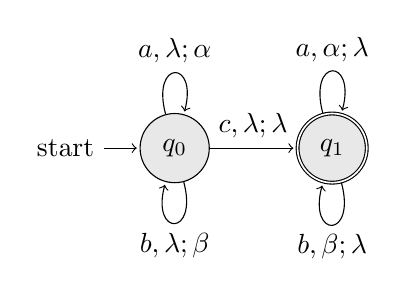
\begin{tikzpicture}[shorten >=1pt,node distance=2cm,on grid,auto]
       \tikzstyle{every state}=[fill={rgb:black, 1;white,10}]

       \node[state, initial] (s_0) {$q_0$};
       \node[state, accepting](s_1) [right of=s_0] {$q_1$};

       \path[->]
       (s_0) edge [loop above] node {$a,\lambda;\alpha$} ()
             edge [loop below] node {$b, \lambda; \beta$} ()
             edge [] node {$c, \lambda ; \lambda$} (s_1)
       (s_1) edge [loop above] node {$a,\alpha;\lambda$} ()
             edge [loop below] node {$b, \beta; \lambda$} ();
     \end{tikzpicture}
     \caption{pushdown automaton accepting $L = \{\textbf{w}c\textbf{w}^r \mid \textbf{w} \in \{a, b\}^*\}$}
   \end{figure}
   
   \item Show that the class of languages accepted by PDA's is closed under
     union, concatenation and and the Kleene star.\\\\
     We will show this by construction of new PDA's. Assume the PDA $M_L =
     \langle \Sigma, \Gamma, Q, q_0, \Delta, F \rangle$ accepts the language $L$
     and $M_{L'} = \langle \Sigma', \Gamma', Q', q'_0, \Delta', F' \rangle$
     accepts $L'$.\\

     First we construct a PDA which accepts $L \cup L'$. $M_{L \cup L'} =
     \langle \Sigma \cup \Sigma', \Gamma \cup \Gamma', Q \uplus Q' \cup \{q''_0\},
     q''_0, \Delta'', F \cup F' \cup \{q''_0\} \text{ if $q_0$ or $q'_0$ is final}
     \rangle$ where $\Delta'' = \Delta \cup \Delta' \cup \{(q''_0, a, \alpha ;
     \beta, q_i) \mid (q_0, a, \alpha ; \beta, q_i) \in Q \lor (q'_0, a, \alpha
     ; \beta, q_i) \in Q'\}$.
     That is a PDA whose alphabet and stack alphabet are simply the union of the
     original PDAs'. In the set of states take a disjoint union and add a new
     initial state $q''_0$. This is also in $F''$ if either original initial state was final.
     Finally we add rules to go from the new initial state to all states
     reachable from original initial states. This is straight-forwardly analogous to the
     construction of $M_{L \cup L'}$ for finite automata.\\
     This new PDA accepts all the words in $L$ because paths through $M_L$ are
     also in $M_{L \cup L'}$. It accepts the words in $L'$ by the same argument.
     It does not accept any other words because any path from $q''_0$ to a final
     state is also a path from either $q_0$ or $q'_0$ to a final state, with the
     first swapped for one of the new added steps and hence must be in $L$ or
     $L'$.\\

     To construct a PDA which accepts $L \cdot L'$ we ``append'' one PDA
     to the other by adding rules $\{(q_i, a, \alpha ; \beta, q'_0) \mid (q_i,
     a, \alpha, \beta, q_j) \in \Delta \land q_j \in F\}$ and letting $F'$ be
     the final states. Additionally, if $q'_0$ is final, each $q_i$ should also
     be made final. Again, this is analogous to the construction of finite
     automata for concatenation of regular languages.\\

     Finally, the Kleene star of a language $L^*$ is accepted by ``looping''
     $M_L$. To do this we add a new initial and final state $q'_0$ and an ``empty'' rule
     $(q'_0, \lambda, \lambda ; \lambda, q_0)$, allowing our new machine to
     accept the empty word (zero loops). Then add rules $(q_i, a, \alpha; \beta,
     q_0)$ for each rule $(q_i, a, \alpha; \beta, q_j)$ in $M_L$ where $q_j$ is final.
     
\end{itemize}
\section*{Textbook 4.1}
\begin{itemize}[label=]
  \item \textbf{14)} Construct a grammar for the language $(ab)^* \mid (ac)^*$
    \begin{lstlisting}
      S -> abA | acB
      A -> abA | l
      B -> acB | l
      \end{lstlisting}
  \item \textbf{21)} Construct a grammar for the language $(a | b)^*(aa | bb)(a|b)^*$
    \begin{lstlisting}
      S -> aA | bA | B
      A -> aA | bA | B
      B -> aaC | bbC
      C -> aC | bC | l
      \end{lstlisting}
   \item \textbf{24)} Find an automaton which accepts the language generated by
     \lstinline{S -> aB}, \lstinline{A -> aB}, \lstinline{B -> bA | b}\\\\
    We construct an automaton with states $N \cup \{f\}$ and initial state $S$
    following the procedure:
    \begin{itemize}[label=$\cdot$]
    \item \lstinline{A -> aB} becomes the rule $(A, a, B)$
    \item \lstinline{A -> a} becomes the rule $(A, a, f)$
      \item \lstinline{A -> l} makes $A$ final
      \end{itemize}
    \begin{figure}[H]
     \centering
     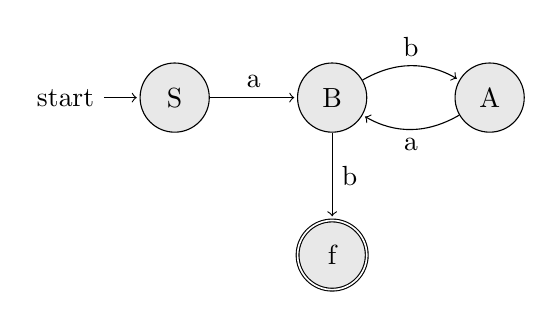
\begin{tikzpicture}[shorten >=1pt,node distance=2cm,on grid,auto]
       \tikzstyle{every state}=[fill={rgb:black, 1;white,10}]

       \node[state, initial] (S) {S};
       \node[state] (B) [right of=S] {B};
       \node[state] (A) [right of=B] {A};
       \node[state, accepting] (f) [below of=B] {f};

       \path[->]
       (S) edge [] node {a} (B)
       (B) edge [bend left] node {b} (A)
       edge [] node {b} (f)
       (A) edge [bend left] node {a} (B);
     \end{tikzpicture}
     \caption{The finite automaton for \textbf{24)}}
     \end{figure}
   \item \textbf{36)} Construct a grammar that generates the language accepted
     by a given finite automaton.\\\\
     We apply the procedure from the previous question in reverse.
     \begin{itemize}[label=$\cdot$]
      \item the rule $(Q, a, Q')$ becomes \lstinline{Q -> aQ'}
      \item if $Q' \in F$, add \lstinline{Q -> a} to our grammar rules
      \item if $Q \in F$, add \lstinline{Q -> l} to our rules
      \end{itemize}
      Also note that the state $S_4$ is a dead end, and will not contribute to
      the accepted language. The resulting grammar has $N = \{S_0, S_1, S_2,
      S_3\}$, $\Sigma = \{a, b\}$ and production rules:
      \begin{itemize}[label=]
      \item $S_0 \rightarrow aS_1 \mid bS_2$
        \item $S_1 \rightarrow bS_1 \mid aS_3 \mid a$
        \item $S_2 \rightarrow aS_1 \mid bS_3 \mid b$
          \item $S_3 \rightarrow \lambda$
        \end{itemize}
  \end{itemize}

  \section*{Textbook 4.2}
  \textbf{4)} and \textbf{5)} concern the grammar $G$ with $N = \{A, B, S\}$,
  $\Sigma = {a, b}$, $R:$
    \begin{lstlisting}
      S -> ABABABA
      A -> Aa | l
      B -> b
      \end{lstlisting}
  \begin{itemize}[label=]
  \item \textbf{4)} convert the grammar to Chomsky Normal Form (CNF).\\
    We proceed in 3 steps:
    \begin{enumerate}
      \item Remove \lstinline{A -> Aa} by constructing the new non-terminal
        $N_a$ and rules \lstinline{$N_a$ -> a, A -> A$N_a$}
      \item Eliminate rules with more than two non-terminals on the right. We
        replace \lstinline{S -> ABABABA} with
        \begin{lstlisting}
S -> A$S_1$
$S_1$ -> B$S_2$
$S_2$ -> A$S_3$
$S_3$ -> B$S_4$
$S_4$ -> A$S_5$
$S_5$ -> BA
        \end{lstlisting}
      \item Get rid of the null production \lstinline{A -> l}
      \end{enumerate}
      The resulting grammar $G' = \langle \Sigma, N \cup \{N_a, S_{1}, ... ,
      S_5\}, S, R' \rangle$ with $R' = $
      \begin{lstlisting}
A -> A$N_a$
$N_a$ -> a
B -> b
S -> A$S_1$
$S_1$ -> B$S_2$
$S_2$ -> A$S_3$
$S_3$ -> B$S_4$
$S_4$ -> A$S_5$
$S_5$ -> BA
\end{lstlisting}

    \item \textbf{5)} convert the grammar to Greibach normal form\\
      Starting with the grammar $G'$ already in CNF we proceed in two steps:
      \begin{enumerate}
        \item Remove the left recursive rule \lstinline{A -> A$N_a$}
      \end{enumerate}
  \end{itemize}
\end{document}
